% TikZ schematic: Quality-Aware Decision Tree
% Standalone version - compile with pdflatex
\documentclass[border=10pt]{standalone}
\usepackage{tikz}
\usepackage{xcolor}
\usetikzlibrary{shapes,arrows,positioning,calc,decorations.pathreplacing,patterns,fit,backgrounds}

\definecolor{inputblue}{RGB}{31,119,180}
\definecolor{fftgreen}{RGB}{44,160,44}
\definecolor{featorange}{RGB}{255,127,14}
\definecolor{arrowgray}{RGB}{100,100,100}

\begin{document}
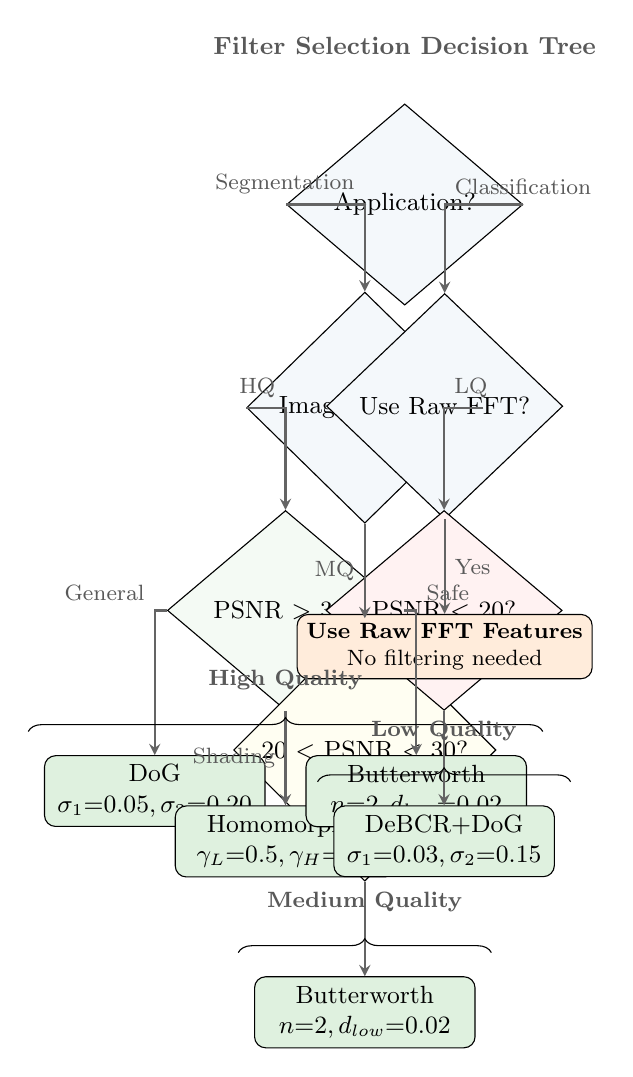
\begin{tikzpicture}[
 node distance=1.2cm and 1.5cm,
 decision/.style={diamond, draw, fill=inputblue!5, minimum width=3cm, minimum height=1cm, align=center, font=\small},
 action/.style={rectangle, draw, fill=fftgreen!15, rounded corners, minimum width=2.8cm, minimum height=0.8cm, align=center, font=\small},
 leaf/.style={rectangle, draw, fill=featorange!15, rounded corners, minimum width=2.5cm, minimum height=0.7cm, align=center, font=\footnotesize},
 arrow/.style={->, >=stealth, thick, color=arrowgray},
 label/.style={font=\footnotesize, color=gray!70!black}
]

% Root
\node[decision] (root) {Application?}; 

% Level 1: Application type
\node[decision, below left=1.2cm and -1cm of root] (app_seg) {Image Quality?}; 
\node[decision, below right=1.2cm and -1cm of root] (app_class) {Use Raw FFT?}; 

% Segmentation branch - Level 2
\node[decision, below left=1.2cm and -0.5cm of app_seg, fill=fftgreen!5] (seg_hq) {PSNR $>$ 30?}; 
\node[decision, below=1.2cm of app_seg, fill=yellow!5] (seg_mq) {20 $<$ PSNR $<$ 30?}; 
\node[decision, below right=1.2cm and -0.5cm of app_seg, fill=red!5] (seg_lq) {PSNR $<$ 20?}; 

% Segmentation branch - Level 3 (HQ)
\node[action, below left=1.2cm and -0.5cm of seg_hq] (hq_dog) {DoG\\$\sigma_1{=}0.05, \sigma_2{=}0.20$}; 
\node[action, below=1.2cm of seg_hq] (hq_homo) {Homomorphic\\$\gamma_L{=}0.5, \gamma_H{=}2.0$}; 
\node[action, below right=1.2cm and -0.5cm of seg_hq] (hq_butter) {Butterworth\\$n{=}2, d_{low}{=}0.02$}; 

% Segmentation branch - Level 3 (MQ)
\node[action, below=1.2cm of seg_mq] (mq_butter) {Butterworth\\$n{=}2, d_{low}{=}0.02$}; 

% Segmentation branch - Level 3 (LQ)
\node[action, below=1.2cm of seg_lq] (lq_enhance) {DeBCR+DoG\\$\sigma_1{=}0.03, \sigma_2{=}0.15$}; 

% Classification branch - Level 2
\node[leaf, below=1.2cm of app_class] (class_yes) {\textbf{Use Raw FFT Features}\\No filtering needed}; 

% Arrows - Root
\draw[arrow] (root) -| node[above left, label] {Segmentation} (app_seg);
\draw[arrow] (root) -| node[above right, label] {Classification} (app_class);

% Arrows - Segmentation
\draw[arrow] (app_seg) -| node[above left, label] {HQ} (seg_hq);
\draw[arrow] (app_seg) -- node[left, label] {MQ} (seg_mq);
\draw[arrow] (app_seg) -| node[above right, label] {LQ} (seg_lq);

% Arrows - HQ Segmentation
\draw[arrow] (seg_hq) -| node[above left, label] {General} (hq_dog);
\draw[arrow] (seg_hq) -- node[left, label] {Shading} (hq_homo);
\draw[arrow] (seg_hq) -| node[above right, label] {Safe} (hq_butter);

% Arrows - MQ Segmentation
\draw[arrow] (seg_mq) -- (mq_butter);

% Arrows - LQ Segmentation
\draw[arrow] (seg_lq) -- (lq_enhance);

% Arrows - Classification
\draw[arrow] (app_class) -- node[right, label] {Yes} (class_yes);

% Braces
\draw[decorate, decoration={brace, amplitude=5pt}]
 ($(hq_dog.north west)+(-0.2,0.3)$) -- ($(hq_butter.north east)+(0.2,0.3)$)
 node[midway, above=0.4cm, label] {\textbf{High Quality}};

\draw[decorate, decoration={brace, amplitude=5pt}]
 ($(mq_butter.north west)+(-0.2,0.3)$) -- ($(mq_butter.north east)+(0.2,0.3)$)
 node[midway, above=0.4cm, label] {\textbf{Medium Quality}};

\draw[decorate, decoration={brace, amplitude=5pt}]
 ($(lq_enhance.north west)+(-0.2,0.3)$) -- ($(lq_enhance.north east)+(0.2,0.3)$)
 node[midway, above=0.4cm, label] {\textbf{Low Quality}};

% Title
\node[label, above=0.5cm of root, font=\small\bfseries] {Filter Selection Decision Tree}; 

\end{tikzpicture}
\end{document}
